%-------------------------------------------------------------------------------
%-------------------------------------------------------------------------------
\section*{Introduction}
%-------------------------------------------------------------------------------
%-------------------------------------------------------------------------------

%-------------------------------------------------------------------------------
%-------------------------------------------------------------------------------
\subsection*{Two main questions}
%-------------------------------------------------------------------------------

%------------------------------------------------------------------------------
\frame{ \frametitle{Network analysis}

  \paragraph{Networks} are convenient to describe interactions between a set of entities, i.e.
  \begin{itemize}
    \item genes within a cell, 
    \item microbes within a medium, 
    \item neurones in a brain, 
    \item \dots
  \end{itemize}
  
  $$
  \begin{tabular}{cc}
    \begin{tabular}{c}
      \includegraphics[width=.3\textwidth]{\fignet/im_EcoliBVEM}
    \end{tabular}
    & 
    \begin{tabular}{c}    
      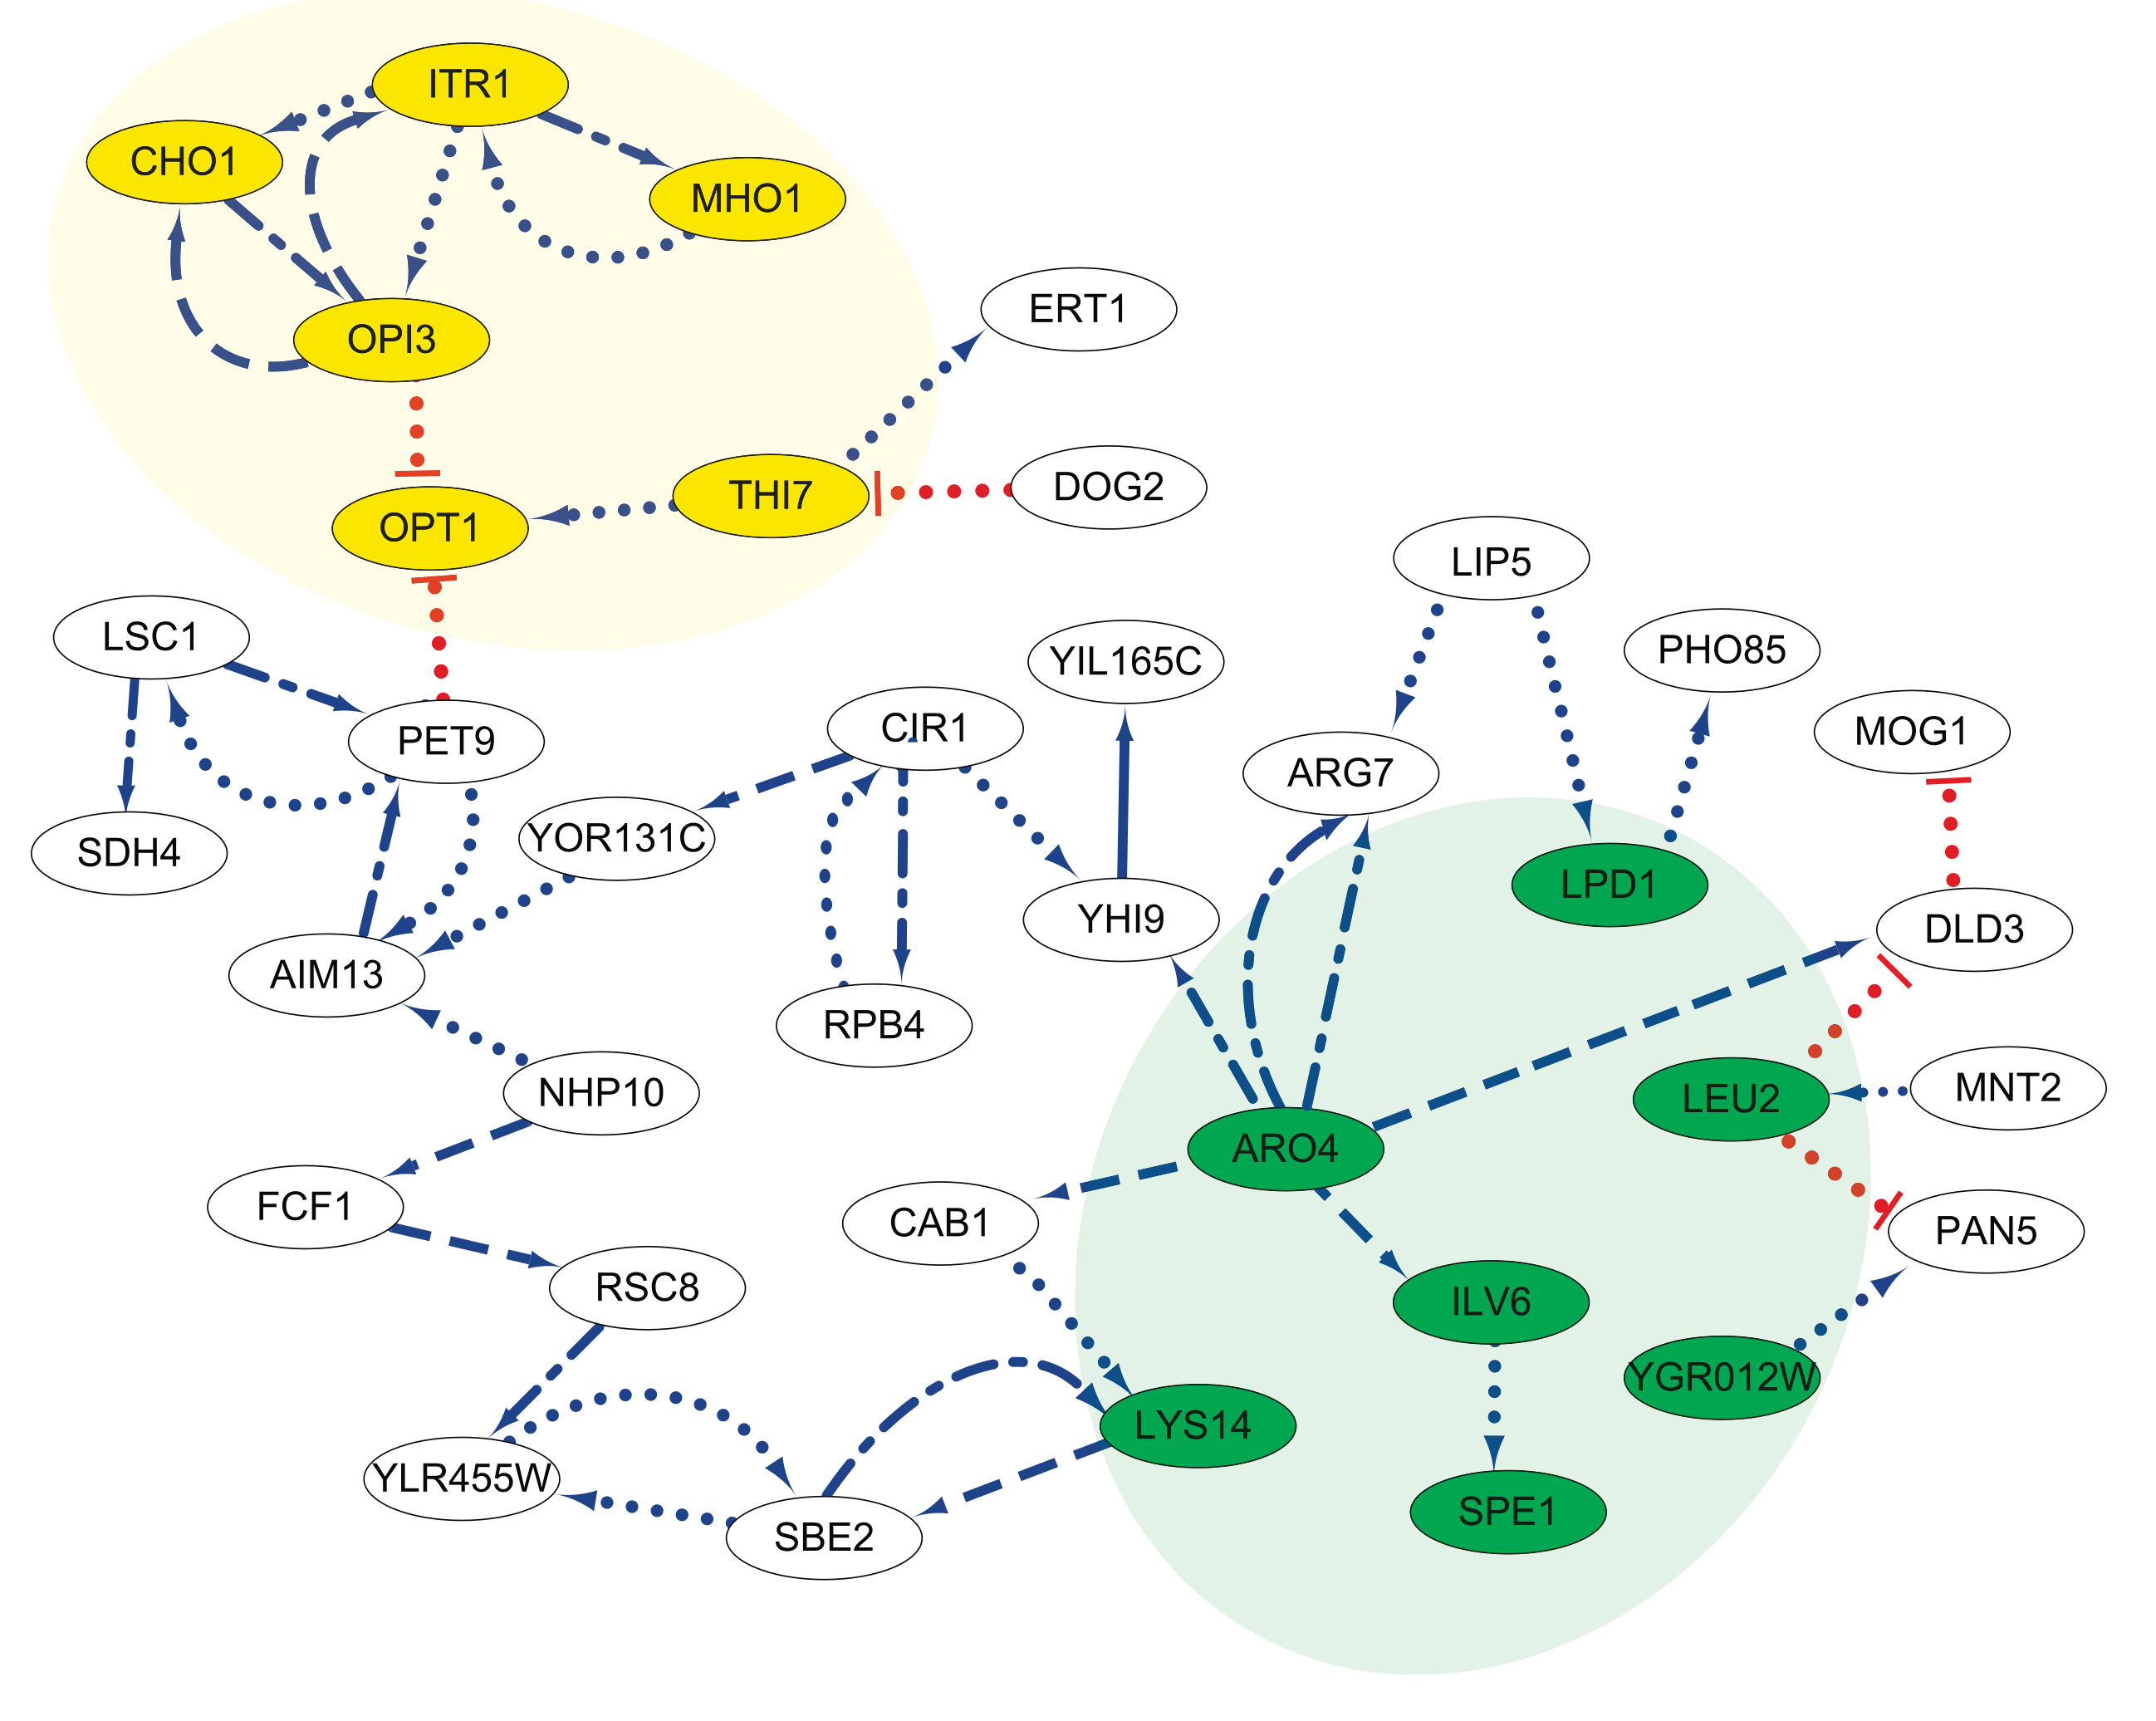
\includegraphics[width=.3\textwidth]{\fignet/CZH19-Nature-Fig1}
    \end{tabular}
  \end{tabular}
  $$
}

%------------------------------------------------------------------------------
\frame{ \frametitle{A bit of vocabulary}

  \paragraph{Definition.} 
  \begin{align*}
    \text{Network} & = \text{ biological object} \\
    \text{Graph} & = \text{ its mathematical representation} \\
  \end{align*}

  \bigskip \pause
  \paragraph{Correspondance.}
  $$
  \begin{tabular}{ccc}
    Network & & Graph $G = (V, E)$ \\
    \hline
    Entity (gene, microbe, neurone, \dots) & $=$ & Vertex (or node) \\
    'Interaction' & $=$ & Edge 
  \end{tabular}
  $$
  
  \bigskip \pause
  Depending on the type of interaction, edges can be 
  \begin{itemize}
   \item binary (presence/absence) or valued (weighted), 
   \item undirected or directed, 
   \item univariate or multivariate, 
   \item \dots
  \end{itemize}
  
}

%------------------------------------------------------------------------------
\frame{ \frametitle{Observed network}

  \begin{tabular}{cc}
    \hspace{-.04\textwidth}
    \begin{tabular}{p{.5\textwidth}}
        \paragraph{Observed network.} \\
        'Interaction' between each pair of entities have been observed or tested, in a experimental manner (think of protein-protein interactions)
        
        \bigskip \bigskip 
        \paragraph{Questions:} 
        \begin{itemize}
        \item How does the system work?
        \item How is is organized?
        \item Do some entities play a specific role?
        \item \dots
        \end{itemize}
    \end{tabular}
    & 
    \begin{tabular}{c}
      \includegraphics[width=.4\textwidth]{\fignet/im_EcoliBVEM}
    \end{tabular}
  \end{tabular}

}

%------------------------------------------------------------------------------
\frame{ \frametitle{Network not observed}

  \begin{tabular}{cc}
    \hspace{-.04\textwidth}
    \begin{tabular}{p{.5\textwidth}}
        \paragraph{Network not observed.} \\
        Information have been collected on each entity (think of gene expression)
        
        \bigskip \bigskip 
        \paragraph{Questions:} 
        \begin{itemize}
        \item How to define an 'interaction'?
        \item Can we 'reconstruct' the network?
        \item How to validate the results?
        \item \dots
        \end{itemize}
    \end{tabular}
    & 
    \begin{tabular}{c}
      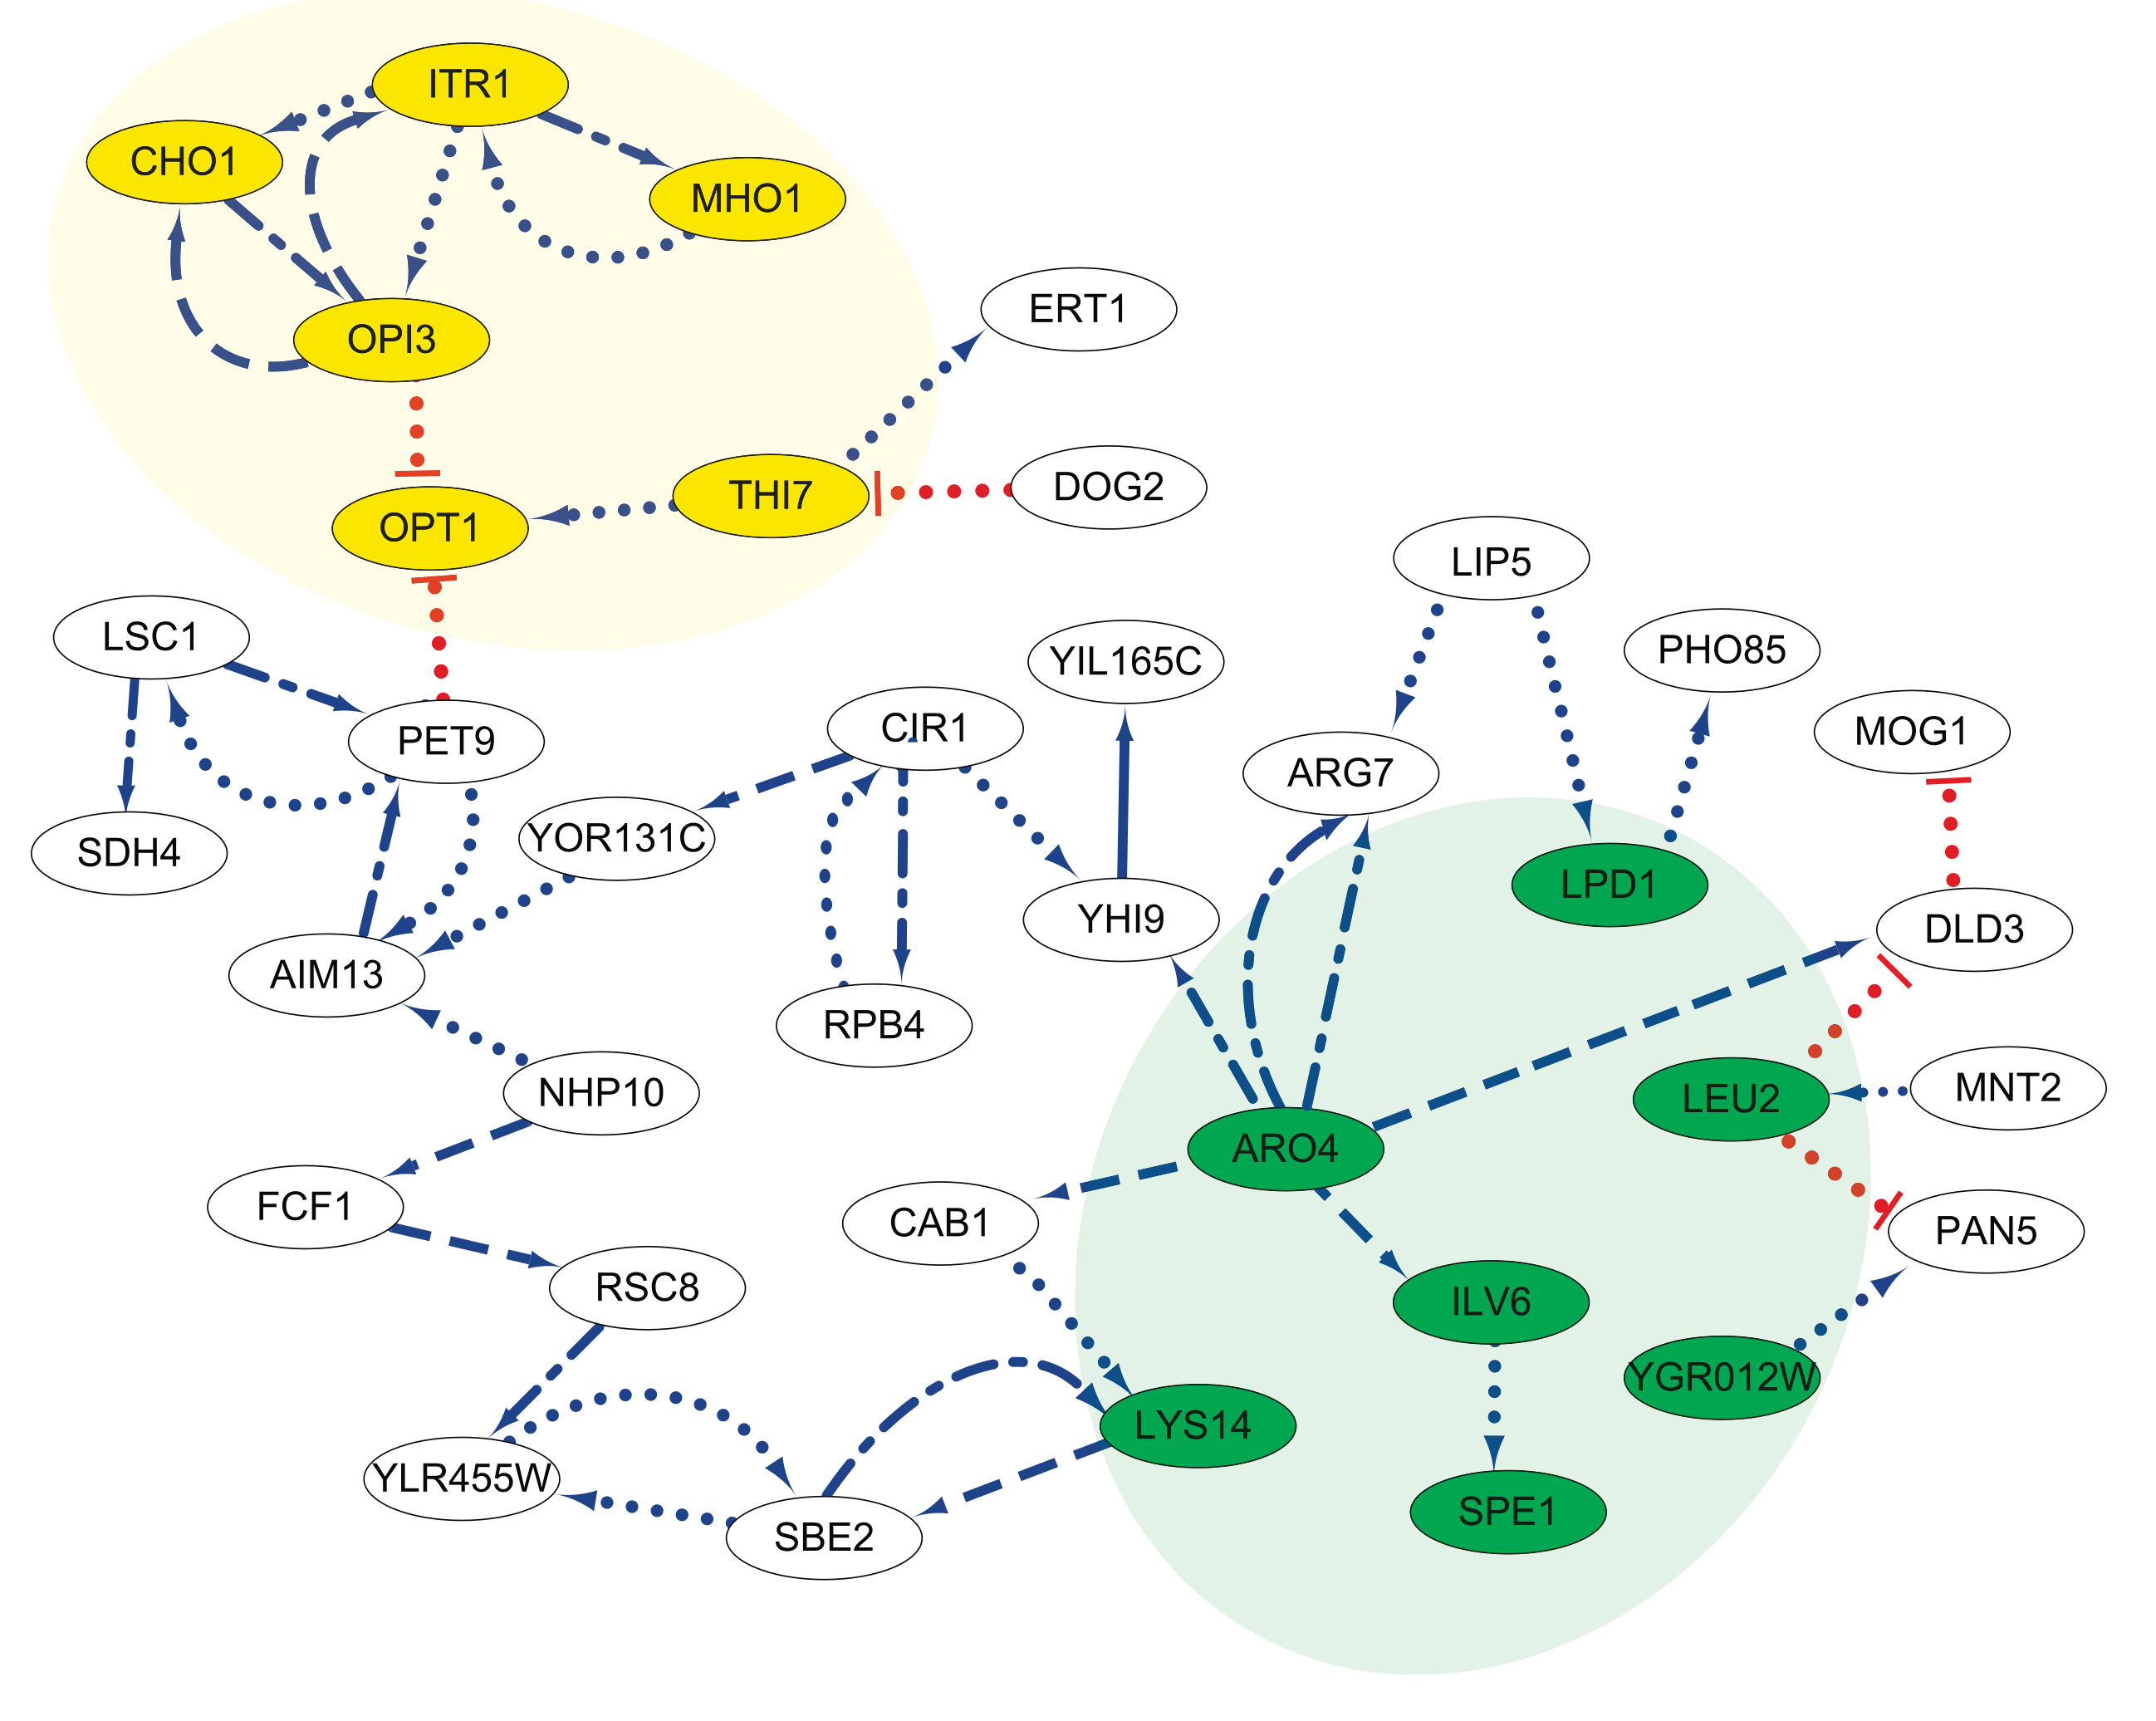
\includegraphics[width=.4\textwidth]{\fignet/CZH19-Nature-Fig1}
    \end{tabular}
  \end{tabular}

}

% %------------------------------------------------------------------------------
% \frame{ \frametitle{Two main situations}
% 
%   \paragraph{Network not observed:} 
%   we aim at reconstructing it
%   $$
%   \rightarrow \text{'network inference'}
%   $$
%   
%   \bigskip \bigskip \pause
%   \paragraph{Observed network:} 
%   we aim at understanding it
%   $$
%   \rightarrow \text{'network analysis'}
%   $$
% }
% 
